\documentclass[../PS6_RapportFinal.tex]{subfiles}

\begin{document}
\graphicspath{{img/}{tex/img/}}

\subsection{Mesures des caractéristiques thermiques du compost}
\label{mesurecaracteristiques}

\subsubsection{Mesure de la conductivité}

La mesure de cette caractéristique est nécessaire pour alimenter l'algorithme qui modélise le comportement thermique de la cuve, on va employer plusieurs méthodes dans le but de vérifier la cohérence des résultats, les mesures étant incertaines à cause de l'hétérogénéité du matériau.

\subsubsubsection{Avec un conductivimètre}

\paragraph{}
On se sert d'un conductivimètre mis à disposition au laboratoire de génie civil. On néglige les effets de bords car on considère que l'échantillon est relativement grand par rapport à l'échelle du modèle.


\begin{figure}[h]
\centering

% Exp 1
\begin{minipage}[h]{7cm}
\centering
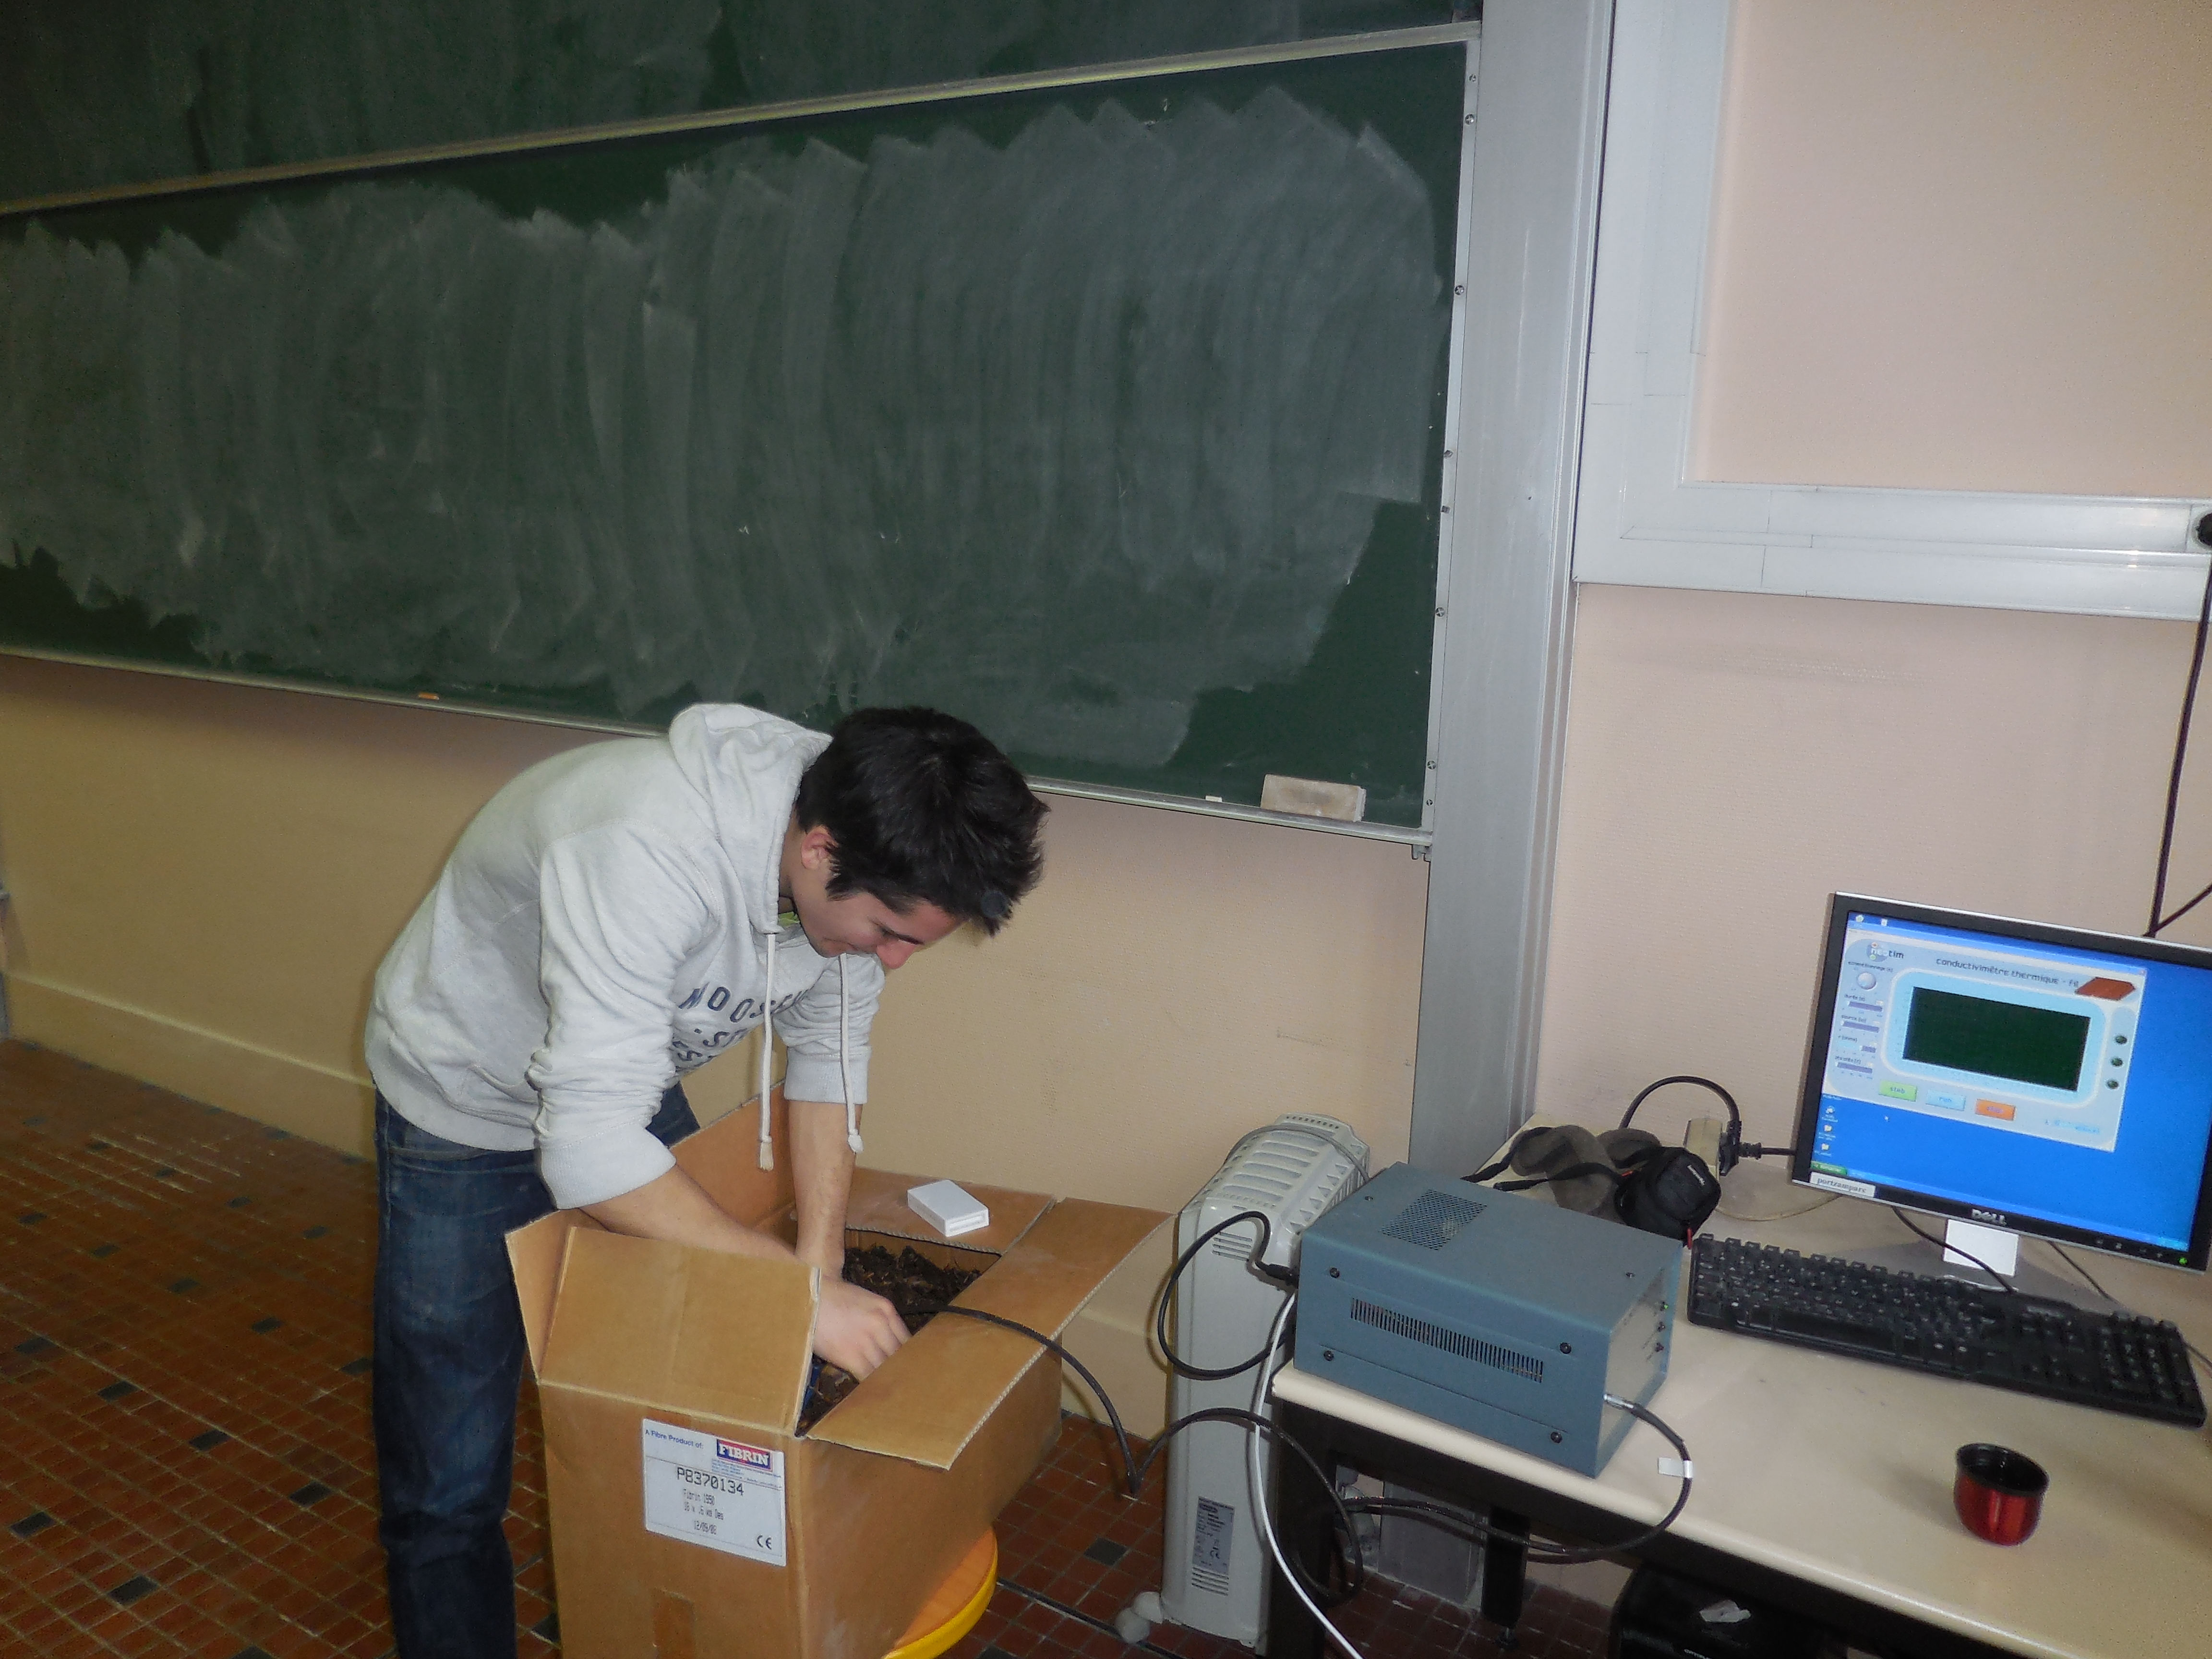
\includegraphics[width=7cm]{2_3_ConductivimetreA.jpg}
\caption{Dispositif de mesure}
\end{minipage}
\hfill
% Experience 2
\begin{minipage}[h]{7cm}
\centering
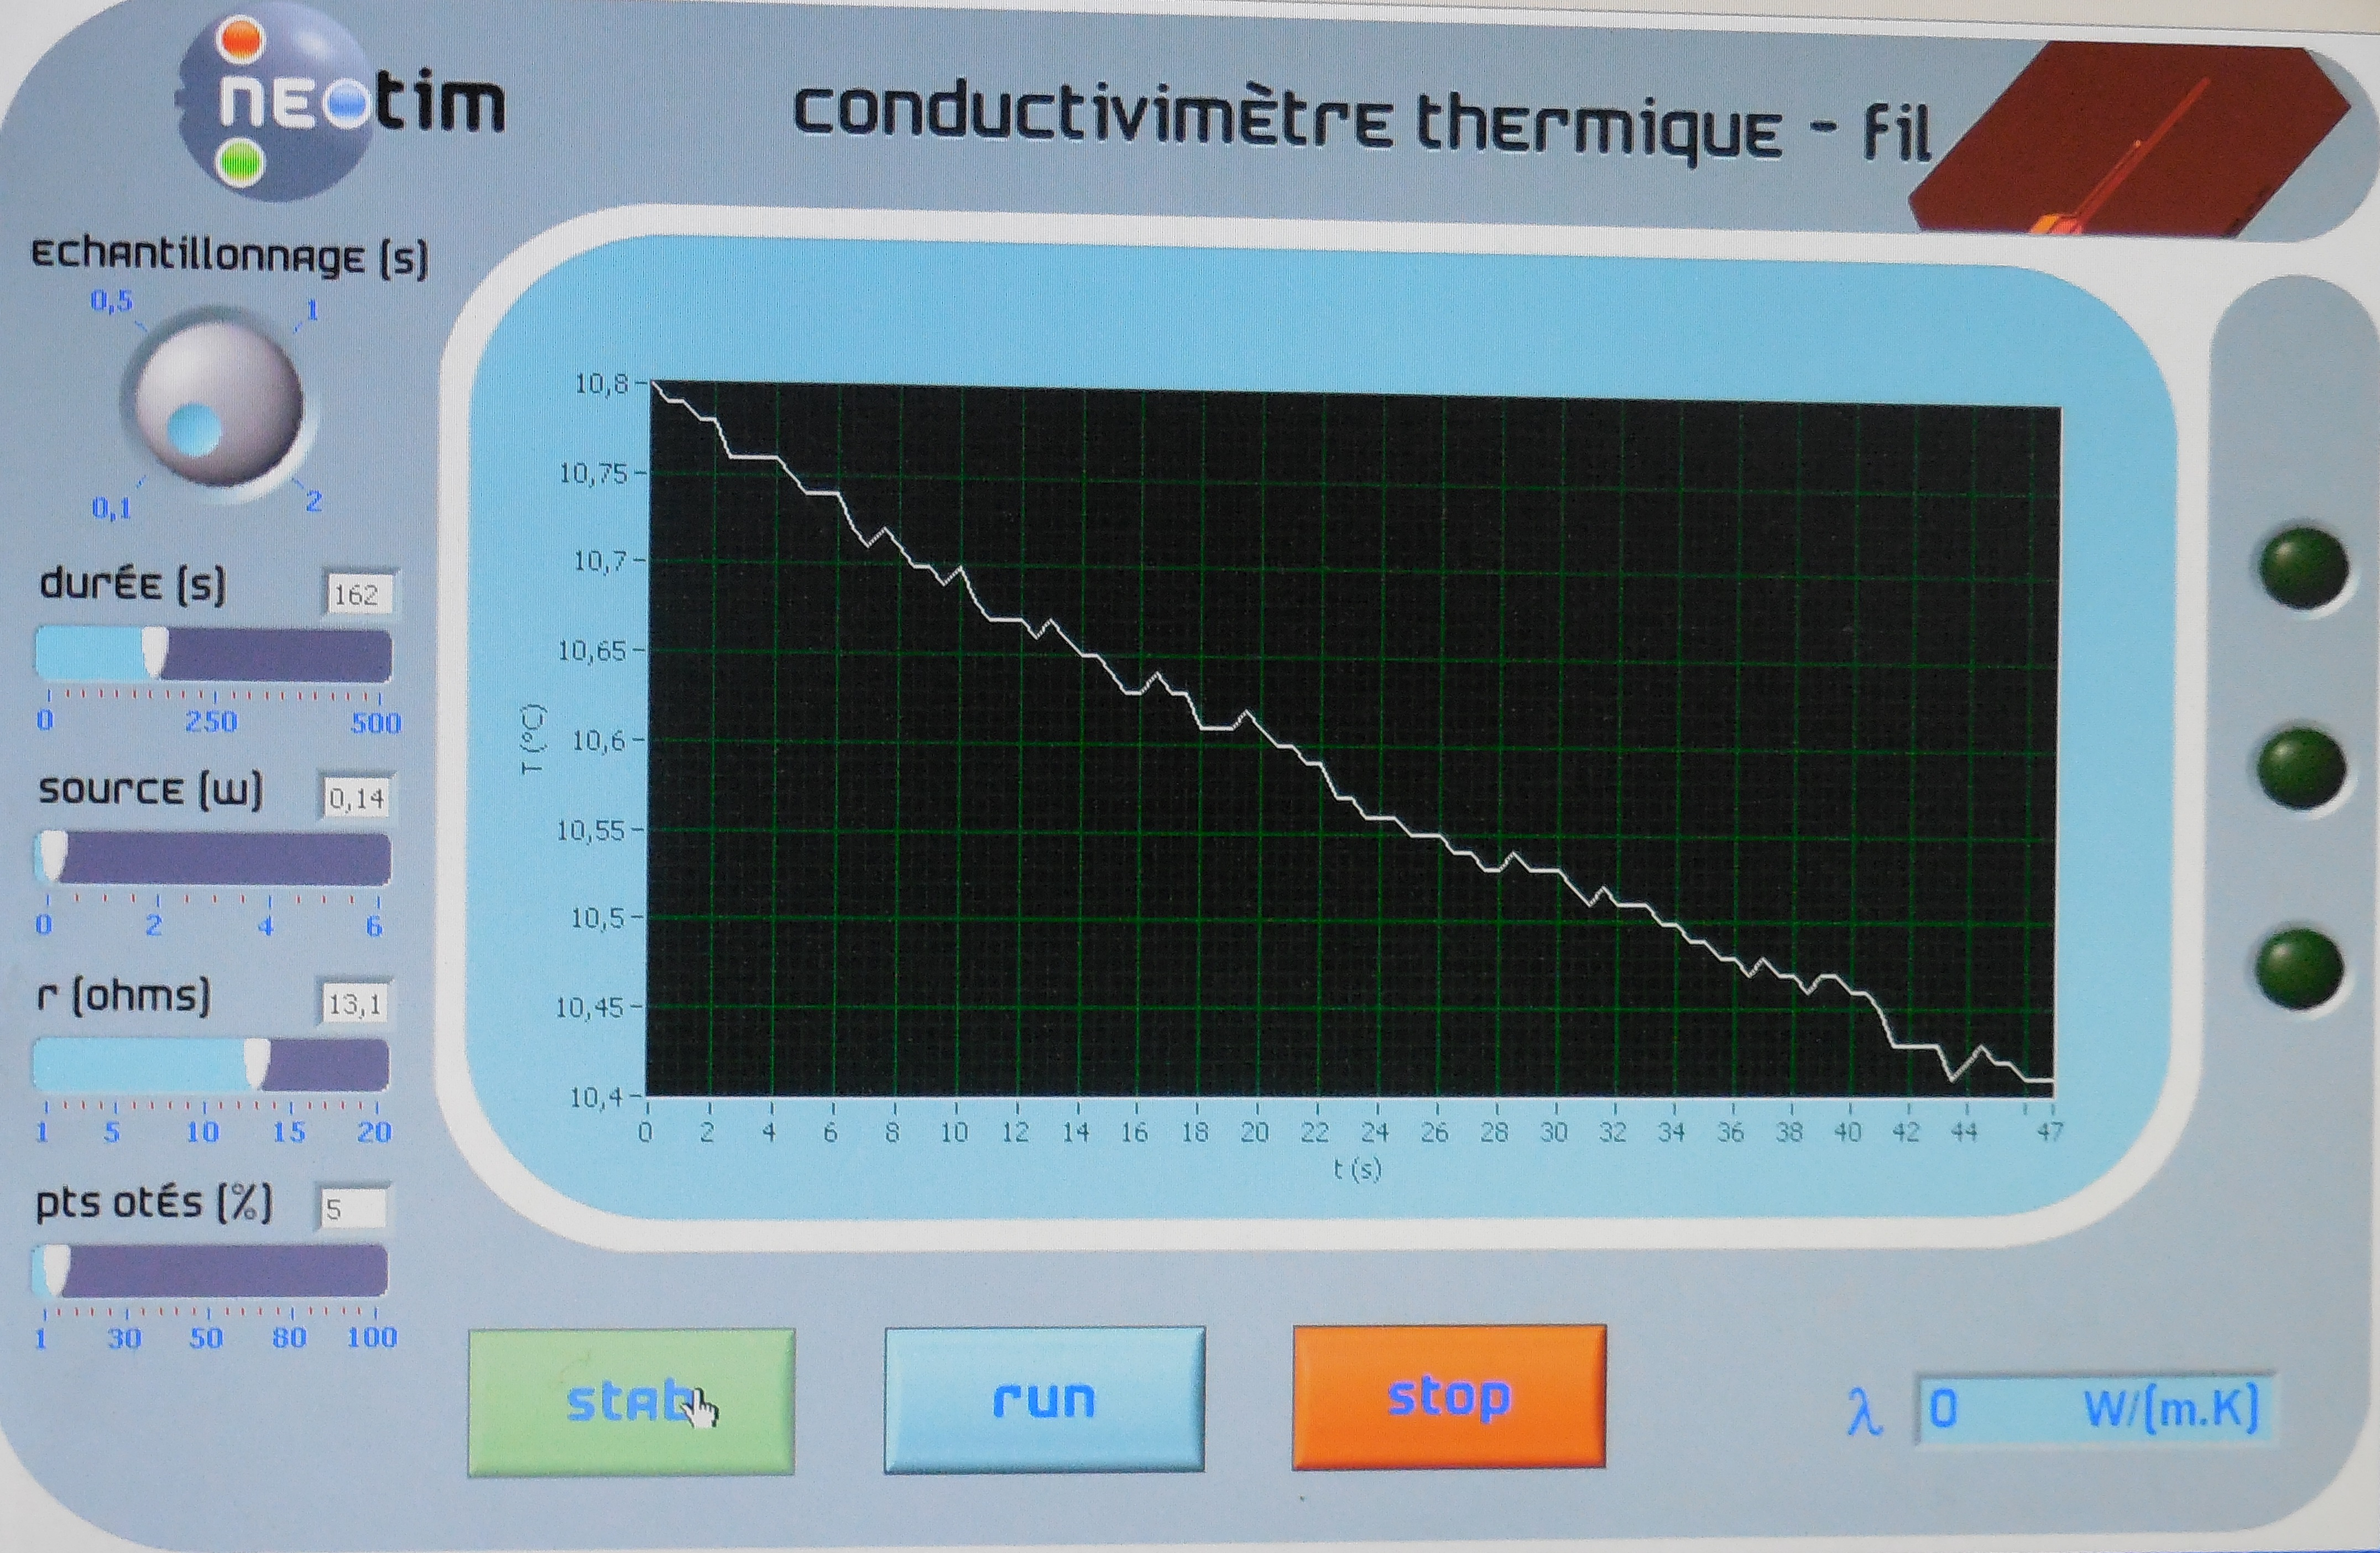
\includegraphics[width=7cm]{2_3_ConductivimetreB.jpg}
\caption{Graphe obtenu}
\end{minipage}

\label{mesure_conductivimetre}
\end{figure}

Voici résumé table 1 la mesure avec cet appareil.

\begin{table}[!h]
\begin{center}
\begin{tabular}{|c|c|c|c|}
\hline \textbf{Puissance [$\si{\watt}$]}& \textbf{Pas de temps [$\si{\milli\second}$]} & \textbf{Durée [$\si{\second}$]} & \textcolor{red}{\textbf{Conductivité thermique [$\si{\watt\per\metre\per\kelvin}$]}} \\ 
\hline $\num{0.05}$ & $100$ & $181$ & \textcolor{red}{\textbf{$\num{0.097}$}} \\ 
\hline 
\end{tabular} 
\caption{Récapitulatif de la mesure au conductivimètre}
\label{table_conductivimetre}
\end{center}
\end{table}

La valeur a été obtenue avec une corrélation de \num{0.987}.

\paragraph{Remarque :}
Plusieurs mesures ont confirmé la même valeur de conductivité et, le coefficient de corrélation étant élevé, on peut considérer cette mesure comme fiable.
Pourtant, les mesures qui suivent infirme la véracité de cette considération.

\subsubsubsection{Par fraction volumique}

On considère le compost comme un mélange d’air et de bois humide.  

\paragraph{Protocole :}       
on va insérer du sable fin clair dans le compost, qui va prendre la place occupée par l'air. On effectue ensuite une coupe du compost et on prend une photo. En accentuant le contraste (Figure \ref{fraction_volumique}), on discerne bien la surface coupée correspondant à la place occupée par l'air, de celle occupée par le bois. La méthode de Lattice Boltzmann permet alors de calculer la diffusivité apparente du compost grâce à de la reconnaissance d'image : un algorithme associe sur une bitmap les pixel correspondant au bois auquel il attribue sa diffusivité, et de même pour l'air, et ce à partir de la photo.

\paragraph{Résultat :}
On a alors  \(D = \num{6.6e-8}\si{}\) donc \(\lambda = \num{0.06}\si{\watt\per\square\metre\per\kelvin}\).
 
\begin{figure}[h]
\begin{center}
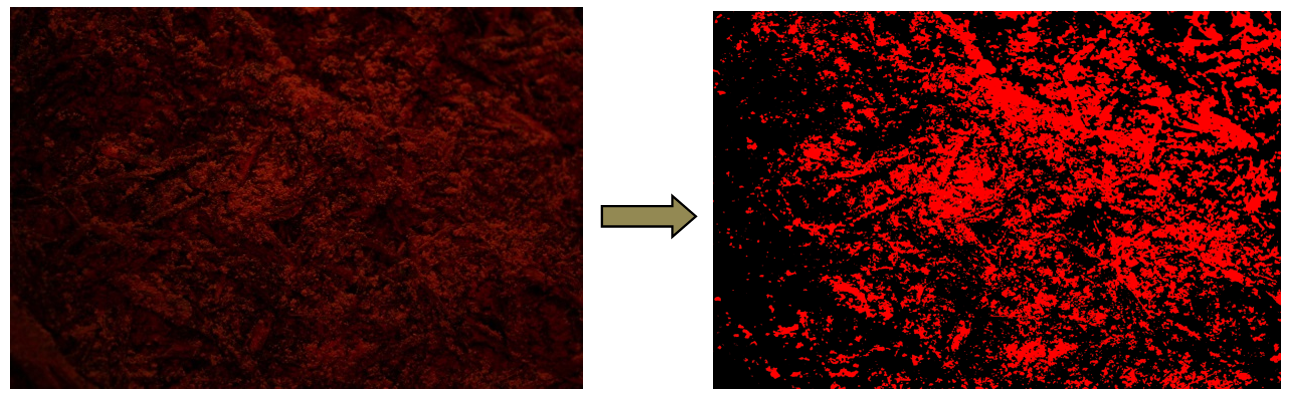
\includegraphics[width=15cm]{2_3_Fraction_volumique.png}
\caption{Photo de la section de compost et de sable (à lumière réelle puis contrastée)}
\label{fraction_volumique}
\end{center}
\end{figure}

\subsubsubsection{Avec un lambdamètre}

On place un échantillon de compost dans une boite puis on fait traverser un flux de chaleur à travers cet échantillon. On déduit la conductivité de la perte de puissance lors de la traversée, perte enregistrée par relevé de température.

\begin{figure}[h]
\centering

% Exp 1
\begin{minipage}[h]{5cm}
\centering
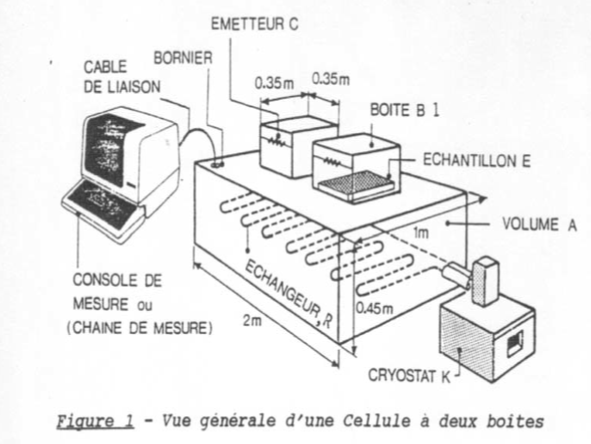
\includegraphics[width=5cm]{2_3_lambdametre2.png}
\end{minipage}
\hfill
% Experience 2
\begin{minipage}[h]{9cm}
\centering
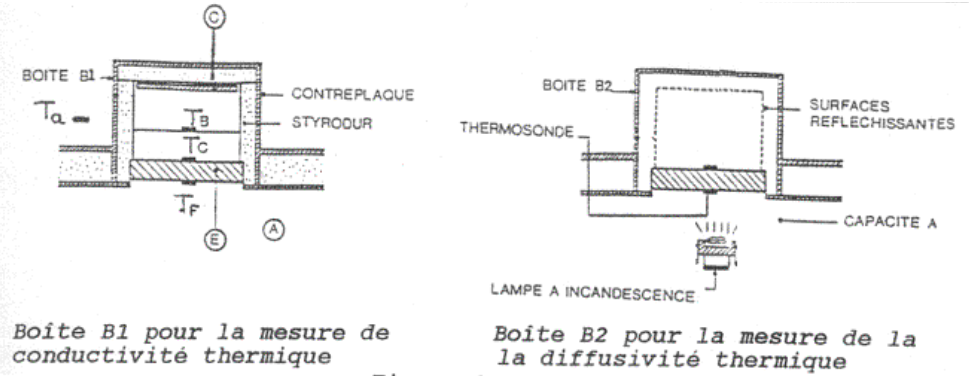
\includegraphics[width=9cm]{2_3_lambdametre.png}
\end{minipage}
\label{mesure_conductivimetre}

\caption{Principe du lambdamètre}
\end{figure}

\begin{figure}[h]

\begin{minipage}[h]{8cm}
	\begin{center}
	\begin{tabular}{|l|c|}
		\hline 
		$V \: [\si{\volt}]$ & $\num{71.8}$ \\
		\hline 
		$R \: [\si{\ohm}]$ & $3253$ \\
		\hline 
		$C$ (constante de cellule) & $\num{0.63}$ \\
		\hline 
		$e \: [\si{\metre}]$ & $\num{0.04}$ \\
		\hline 
		$A \: [\si{\square\metre}]$ & $\num{0.0767}$ \\
		\hline
	\end{tabular}
	\label{parametres_lambdametre}
	\caption{Paramètres du lambdamètre}
	\end{center}
\end{minipage}
\hfill
\begin{minipage}[h]{6cm}
	\begin{center}
	\begin{tabular}{|l|c|}
		\hline 
		$T_{C} \: [\si{\degreeCelsius}]$ & $\num{22}$ \\
		\hline 
		$T_{F} \: [\si{\degreeCelsius}]$ & $\num{31.6}$ \\
		\hline 
		$T_{B} \: [\si{\degreeCelsius}]$ & $\num{17.6}$ \\
		\hline 
		$T_{a} \: [\si{\degreeCelsius}]$ & $\num{16.4}$\\
		\hline
	\end{tabular}
	\label{mesures_lambdametre}
	\caption{Mesures grâce au lambdamètre}
	\end{center}
\end{minipage}
\end{figure}

Toutes ces valeurs sont reliées à la conductivité thermique par la relation suivante :

\begin{equation}
\frac{V^{2}}{R} = A\frac{\lambda}{e}(T_{C}-T_{F})+C(T_{B}-T_{a})
\label{equation_lambdametre}
\end{equation}

On trouve donc $\lambda = \num{0.0538} \: \si{\watt\per\square\metre\per\kelvin}$
Ce qui est cohérent avec la valeur trouvée précédemment.


\subsubsubsection{Conclusion}

En différenciant la formule \ref{equation_lambdametre}, on obtient $\frac{\Delta \lambda}{\lambda} = \num{12.5} \%$.
Cette valeur parait cohérente, aux aléas de mesures près, car on a bien un mélange d'air de conductivité $\lambda = \num{0.01} \: \si{\watt\per\metre\per\kelvin}$ et de bois humide dont la conductivité thermique varie de $\num{0.1}$ à $\num{0.2} \: \si{\watt\per\metre\per\kelvin}$. 

\subsubsection{Mesure de la capacité thermique massique}

\subsubsubsection{Mesure grâce à l'effusivimètre}

Un effusivimètre a également été mis à notre disposition en même temps que le conductivimètre. On pose les mêmes hypothèses où l'on néglige les effets de bord. Une fois l'effusivité $\beta$ connue, et connaissant la conductivité thermique, on peut déduire la capacité thermique grâce à la formule : $ C_{P} = \frac{\beta^{2}}{\rho \gamma}$

\paragraph{Problème :} 
 Contrairement à la mesure de la conductivité, celle de l'effusivité diffère selon les mesures et ne présente pas un bon coefficient de corrélation.On trouve par exemple \(\beta = 218 \) avec un coefficient de correlation de \num{0.77}. La valeur trouvée parait donc erronée et on passe donc par un modèle rhéologique pour trouver une valeur valable de la capacité thermique. 
 

\subsubsubsection{Par fraction massique}


On considère le compost comme un mélange d'eau, de bois et d'air ; on va mesurer ces différentes quantités dans un échantillon, puis effectuer des pondération massiques ou volumiques.



\textbf{Pourcentage d'eau}

\begin{itemize}
\item On prélève un échantillon de compost humide que l'on pèse.
\item On le passe au micro-onde jusqu'à évaporation complète de toute eau.
\item On pèse le compost desséché et on obtient la masse d'eau par soustraction des masses.
\end{itemize}



\textbf{Pourcentage d'air}

\begin{itemize}
\item On place un volume $V$ de compost séché dans un bécher.
\item On remplit ce bécher d'un volume d'eau $V_{eau}$.
\item On mesure le volume $V'$ dans le bécher.
\end{itemize}
On a alors $V_{air} = V + V_{eau} - V'$.
\paragraph{Résultats :}
Le volume d’air est important mais son pourcentage massique est faible car sa densité est négligeable par rapport à celle de l’eau et du bois sec.


On obtient donc
\[
  		\left\{
          \begin{array}{ll}
            \frac{m_{eau}}{m_{total}} = \num{0.54} \\
            \frac{m_{air}}{m_{total}} =  \num{0.0014} \\
            \frac{m_{bois sec}}{m_{total}} =  \num{0.46} \\
          \end{array}
        \right.
\]

Et alors :   $C=\num{0.54}C_{eau}+\num{0.46}C_{bois}=2812 \: \si{\joule\per\metre\per\kilogram}$

\subsubsection{Conclusion}


On a donc pu déterminer les caractéristiques thermiques du compost qui aident à la compréhension globale du phénomène physique et chimique. Ces données servent concrètement à l'élaboration de modèle informatique prédictif de l'évolution de la température à l'intérieur de la cuve.
Pour la conductivité on a retenu la mesure du lambdamètre composée par le modèle rhéologique par fraction volumique.
Pour la capacité thermique massique, on retient le résultat trouvé par décomposition massique du compost.

Bilan   :   
\[
  		\left\{
          \begin{array}{ll}
            \rho = 325 \: \si{\kilogram\per\cubic\metre}\\
            C =  2812 \: \si{\joule\per\kelvin\per\kilogram}\\
            \lambda = 0.0538 \: \: \si{\watt\per\metre\per\kelvin}\\
          \end{array}
        \right.
\]
                       

\end{document}